\section{Stand der Forschung} \label{SdF}

Bevor auf den Stand der Forschung mit den Technologien und Konzepten zur Energieeinsparung eingegangen wird, soll im Folgenden auf relevante Begrifflichkeiten eingegangen werden. Die Begrifflichkeiten sollen zunächst definiert und im Anschluss für die Arbeit abgegrenzt werden.  

\subsection{Begriffe}

\subsubsection{Carrier-Netzwerke}
Gegenstand der Projektarbeit bildet ein hinsichtlich der Energieeffizienz und Wirtschaftlichkeit zu optimierendes Carrier-Netzwerk.

Unter einem Carrier versteht man \textquote{[…] eine Gesellschaft, die mindestens drei Übertra\-gungs\-wege betreibt, die über eine Vermittlungsstelle miteinander verbunden sein müssen} \cite{carrier}. Ein Carrier-Netzwerk stellt somit physikalische Transportwege und -verfahren zur Verfügung und bildet die Grundlage für sogenannte Mehrwertdienste von Providern, welche auf den Carrier-Diensten aufsetzen \cite{fassnacht}. \textquote{Bei den TK-Transportwegen unterscheidet man leitergebundene Verbindungen auf der Basis von Kupferkabeln oder Lichtwellenleitern sowie Funkverbindungen wie Satellitenverbindungen, Richtfunkstrecken und Rundfunkverbindungen} \cite{fassnacht}.

Somit umfasst ein Carrier-Netzwerk nicht nur das physikalische Backbone-Netz, sondern auch das Zugangs- und Aggregationsnetzwerk. Das Kernnetz eines Carriers kann durch ein vereinfachtes Drei-Schichten-Modell dargestellt werden, das sich nach den Protokollschichten für Glasfaser, Ethernet und Internet richtet. 

\subsubsection{Effizienz im Bereich von Telekommunikationsnetzen}
Die Begriffe Energieverbrauch und Energieeffizienz werden in der Literatur häufig gemischt verwendet. Während es auf der einen Seite notwendig ist, den Energieverbrauchs zu reduzieren, muss auf der anderen Seite auch die Kapazität und Performanz eines Netzwerks erhalten werden. Energieeffiziente Konzepte und Technologien zielen also darauf ab, den Energieverbrauch pro übertragener Datenmenge so gering wie möglich zu halten. \cite{aleksic2013}

Um die Energieeffizienz zu definieren soll folgende Formel verwendet werden:

\begin{equation}
E_{eff}=\frac{N_{user}*R_{user}}{P_{total}}
\end{equation}

$E_{eff}$ steht für die Menge des übertragenen Datenverkehrs pro Energieeinheit, während $P_{total}$ den gesamten Energieverbrauch des zu betrachtenden Netzwerks beziffert. $N_{user}$ gibt die Zahl der aktiven Nutzer im Netzwerk an und $R_{user}$ die verfügbare Datenrate je Nutzer. \cite{aleksic2013}
Die Formel drückt das Verhältnis der übertragenen Datenmenge zur benötigten Leistung aus.

\subsubsection{Wirtschaftlichkeit}
Bei der Betrachtung von Energiesparpotentialen in Netzwerken findet die Wirtschaftlichkeit häufig keine Beachtung. Die Wirtschaftlichkeit drückt aus, wie sparsam mit vorhandenen Ressourcen umgegangen wird.  Vor jeder Investition steht die Frage nach der betriebswirtschaftlichen Sinnhaftigkeit. Im ökonomischen Sinn bedeutet Wirtschaftlichkeit das Verhältnis aus monetären Kosten und Leistung. Die Wirtschaftlichkeit kann mit folgender Gleichung definiert werden:

\begin{equation}
Wirtschaftlichkeit=\frac{Ertrag (bzw. Leistung)}{Aufwand(bzw. Kosten)}
\end{equation}


Für die Wirtschaftlichkeitsbetrachtung in dieser Arbeit werden die Ausgaben für die Anschaffung der Netzwerkkomponenten (englisch: Capital Expenditures, kurz: Capex) nicht be\-rück\-sich\-tigt. Die für den operativen Geschäftsbetrieb anfallenden Aufwendungen werden \textquote{Operational Expenditures} (kurz: Opex) genannt und stellen die Betriebskosten dar. Zu den laufenden Ausgaben für den Geschäfts\-betrieb gehören u.a. Mieten, Personal- und Energiekosten, Aufwendungen für Wartung und Support sowie Verbrauchsmaterialien und Betriebsstoffe. In den folgenden Kapiteln der Arbeit sollen Berechnung der Wirtschaftlichkeit die reinen Betriebskosten, also der Stromverbrauch, der für den Betrieb der Hardware anfällt, betrachtet werden. Ausgenommen davon sind die Kosten, die durch Kühlung der Hardware anfallen. 


\subsection{Technologien und Konzepte zur Reduzierung des Energieverbrauchs in Telekommunikationsnetzwerken}
In diesem Kapitel sollen Konzepte vorgestellt werden, die der Einsparung von Energie in Netzwerken dienen können, sowie Technologien und Entwicklungen erläutert werden, welche die genannten Konzepte umsetzen. Möglichkeiten zur Steigerung der Energieeffizienz bzw. Reduzierung des Energieverbrauchs in einem Telekommunikationsnetzes können wie folgt unterteilt werden:
\begin{itemize}
	\item Energieeffiziente Netzelemente
	\item Energieeffiziente Netzarchitektur
	\item Verkehrslastadaptiver Netzbetrieb
	\item Hybrid Optical Switching
	\item Adaptive Optical Switching
\end{itemize}

\subsubsection{Energieeffiziente Netzelemente}
Durch den technologischen Fortschritt können Netzwerkkomponenten energieeffizienter gestaltet werden, beispielsweise durch zunehmende Integration mehrerer einzelner Geräte\-einheiten in einem Verbundgerät. Somit können mehrere Module in einer Einheit zusammengefasst werden ohne die Netzwerkarchitektur zu verändern. Betrachtet man einzelne Geräte kann durch den Austausch alter Hardware mit neueren, energieeffizienteren Komponenten eine Einsparung erzielt werden. 

\subsubsection{Energieeffiziente Netzarchitektur}
Ein Ansatz bezieht sich auf das Konzept der energieeffizienten Netzwerkarchitektur und sieht eine Vereinfachung des Netzes vor, welche durch eine  Aufteilung des Netzes in Bereiche mit differenzierte geografischer Ausdehnung (Global - Kontinental - National - Regional - Zugang) erfolgen kann \cite{aleksic2014}. Durch das Einteilen des Netzes in Zonen und Einsetzen von adäquaten Übertragungs\-technologien innerhalb der Abgrenzungen können die Einsparpotentiale unabhängig voneinander betrachtet werden.

\subsubsection{Verkehrslastadaptiver Netzbetrieb}
Durch den in der Einleitung erwähnten zunehmenden Datenverkehr und dem daraus resultierenden notwendigen Netzausbau führt eine nahezu konstante Leistungsaufnahme der Netzelemente zu einem Anstieg des Netzenergiebedarfs. Da jedoch die Verkehrslast des Netzes zeitlich variiert, können in Phasen geringerer Last einzelne Systeme in einem Modus mit niedrigerer Leistungsaufnahme betrieben werden, ohne dass eine Beeinträchtigung für die Nutzer entsteht.

Heutige Telekommunikationsnetze werden auf Basis einer Spitzenlast zuzüglich einer Reserve dimensioniert. Für die Dimensionierung der Netze stellt eine dynamische Anpassung der Netzkapazität an die Verkehrslast eine attraktive Lösung dar \cite{lange}.

Tageszeitabhängige Schwankungen der Netzauslastung ermöglichen eine unabhängige und dynamische Abschaltung von Ports und Links unter der Be\-rück\-sich\-ti\-gung der Quality of Service-Bedingungen \cite{aleksic2013}. Dabei werden Algorithmen zur Identifikation von individuell abschaltbaren Links verwendet \cite{fassnacht}. \textcite[1]{fisher} merken an, dass die durchschnittliche Verbindungsauslastung der Backbone-Netzwerke vieler großer Internet Service Provider geschätzt 30 bis 40 Prozent betrage. Abbildung \ref{fig:Netzdimensionierung} zeigt die beiden Prinzipien der Netzdimensionierung.

\begin{figure}[htb]
	\centering
	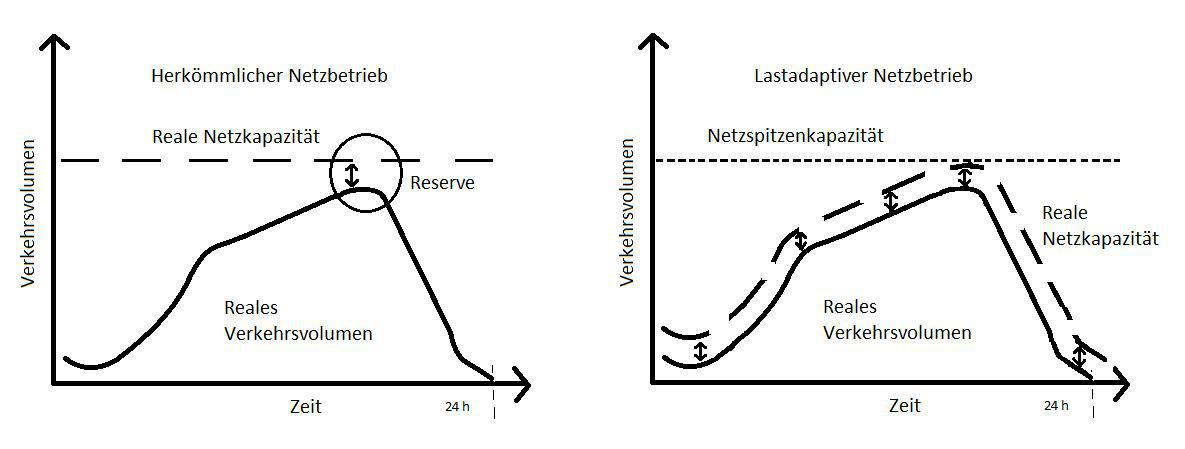
\includegraphics[width=0.8\textwidth]{Netzdimensionierung}
	\caption{Prinzipien der Netzdimensionierung, nach \cite{fisher}}
	\label{fig:Netzdimensionierung}
\end{figure}

Das linke Diagramm \textquote{Herkömmlicher Netzbetrieb} zeigt Verkehrsvolumen in einem Netz, dessen Kapazität aufgrund einer Spitzenlast zuzüglich einer Reserve dimensioniert wurde. Es ist erkennbar, dass die reale Netzkapazität im Laufe eines Tages nur einmal annähernd erreicht wird. Je geringer der Abstand zwischen der Geraden der realen Netzkapazität und dem Graphen ist, desto effizienter ist das Netz. Durch die statische Netzkapazität ist ein konstanter Energieaufwand notwendig, um das Netz zu betreiben. 
Im rechten Diagramm \textquote{Lastadaptiver Netzbetrieb} ist zu erkennen, wie sich die reale Netzkapazität dem realen Verkehrsvolumen anpasst. Die Verläufe der Graphen sind bis auf eine vorgehaltene Reserve gleich. Betrachtet man beide Teile der Grafik, ist zu erkennen, dass die Fläche zwischen der Geraden und dem Graphen beim lastadaptiven Netzbetrieb um einige Vielfache kleiner ist als bei dem statisch dimensionierten Netz. Somit ist das Netz wesentlich effizienter.

Durch die Abschaltung einzelner Ports kann laut der Deutschen Telekom AG der Energiebedarf einiger Elemente um ein Drittel gesenkt werden \cite[4]{lange}. Demnach verbrauchen Ports, die keinen Verkehr leiten, signifikant weniger Energie als solche unter Last. Weiterhin wird beschrieben, dass durch die Deaktivierung ganzer Line Cards und Port Groups per Management System theoretisch 100 Prozent Einsparung erreicht werden kann. In  \cite{lange} wird beschrieben, dass das Deaktivieren der Line Cards im Jahr 2010 nur per manuellen Eingriff mit einem Network Management System erfolgen konnte. Der Aufwand für das dynamische temporäre Abschalten stand  nicht im Verhältnis zur Einsparung. Die Herausforderungen der Hersteller bestanden unter anderem darin, Deaktivierungs- und Aktivierungszeiten der Netzwerkelemente zu reduzieren. Außerdem mussten die Betriebssysteme großer Routersysteme für die genannte Dynamik kompatibel gemacht werden, da Softwarelösungen eine temporäre Aus- und Abschaltung nicht vorsahen.
Heutige Implementierungen in Netzwerkkomponenten, wie zum Beispiel mit dem Dynamic Link Metric Algorithmus, ermöglichen die Abschaltung von 20\% der Anzahl der Verbindungen eines Routing-Elements. Dadurch können 140 Watt pro Gerät eingespart werden\cite{keiouniversity}. Die Idee hinter dem genannten Algorithmus ist, den Datenverkehr auf den meist genutzten Verbindungen zu aggregieren und die dadurch freiwerdenden Verbindungen abzuschalten\cite[592]{survey2013} 


\subsubsection{Hybrid Optical Swiching}
Optische leitungsvermittelnde Switche basieren auf mikro-elektromechanischen Systemen, die eine geringe Menge an Energie benötigen und eine hohe Portanzahl besitzen. Hybrid Optical Switching (HOS) verwendet eine Kombination aus optischen und elektronischen Netzknoten. Zum einen wird \textquote{Optical Circuit Switching} (OCS) verwendet, das laut \textcite{tsinghua2011} als fortgeschrittene und viel verwendete Technologie zur Übermittlung in optischen Netzwerken eingesetzt wird. OCS ist gut geeignet für langanhaltende und kontinuierliche Datenströme, jedoch kommt die Technik bei einem stoßweisen Anstieg des Durchsatzes an ihre Grenzen. Zum anderen wird \textquote{Optical Burst Switching} (OBS) eingesetzt, das für kurzzeitig ansteigende Datendurchsätze optimiert ist. Ein Nachteil der Technik ist die abnehme Leistung bei lang andauernden, kontinuierlichen Strömen. Weiterhin stellt OBS eine hohe Bandbreitennutzung her, benötigt hierfür aber große optische Pufferspeicher. Um effektiv beide Varianten der Datenströme zu übertragen, können mit der Kombination von OCS und OBS die Vorteile beider Technologien verbunden werden. Somit sind die beiden Technologien als komplementäre Ansätze anzusehen \cite{tsinghua2011}. In einem HOS-Netzwerk werden große Datenströme durch vorgehalte Leitungen oder mit langen Durchsatzstößen übertragen und kleinere Ströme durch einzelne Datenpakete und kurze Durchsatzstöße übermittelt. Laut \textcite{adaptiveHOS} hat HOS in den letzten Jahren eine besondere Bedeutung erfahren, da es die gesamte Netzwerkperformanz erhöht und ein erhebliches Energieeinsparpotential beinhaltet.

\subsubsection{Adaptive Optical Swiching}
Das Adaptive Hybrid Optical Switching (AHOS) basiert auf HOS und erweitert das Basiskonzept der Technologie. Das Grundkonzept von AHOS sieht vor, die optische und elektronische Switching-Technologie auf eine effiziente Art zu verwenden, um die Daten optimal zu übertragen. Dabei werden die beiden Technologien von HOS in unterschiedlichen, zeitlichen Rahmen verwendet und die adäquate Methode zur Übertragung der unterschiedlichen Arten der Datenströme ausgewählt. Die Netzwerkknoten in einem AHOS-Netzwerk sind in der Lage, ihren Energieverbrauch abhängig von dem aktuellen Datenverkehr anzupassen. Eine derartige Anpassung ist das temporäre Abschalten von Ports oder Line Cards oder das Aktivieren eines stromsparenden Betriebszustandes \cite{adaptiveHOS}.
